\documentclass[titlepage]{article}
\usepackage{amsfonts}
\usepackage{bbm}
\usepackage{graphicx}
\renewcommand{\baselinestretch}{1}
\usepackage[utf8]{inputenc}
\usepackage{color}
\usepackage[T1]{fontenc}
\usepackage{geometry}
\usepackage{amsmath}
\usepackage{enumerate}
\usepackage{caption}
\usepackage{graphicx}
\usepackage{subcaption}
\usepackage{array}
\usepackage{fullpage}
\usepackage{algorithm2e}
\usepackage{float}
\usepackage{listings}
\everymath{\displaystyle}

\begin{document}
\title{Coach Ranking Model}
\author{Akilesh Potti, Dominick Twitty, Wenhai Yang}
\maketitle

\begin{abstract}
Todo
\end{abstract}



\noindent\textbf{Disclaimer:} For legal and moral reasons, all geographical locations and company names used in this paper are entirely fictional unless otherwise stated. However, for the sake of accuracy, real world data was used to tune our model.


\section{The Problem}
\begin{enumerate}
\item Todo
\end{enumerate}


\section{Model assumptions}
\begin{enumerate}
\item Todo
\end{enumerate}

\section{Models}


\section{Results, Validation, and Robustness}

\begin{figure}[H]
      \centering
      \begin{subfigure}{0.48\textwidth}
	\caption{Distribution of Request Source with Airport}
      \centering
      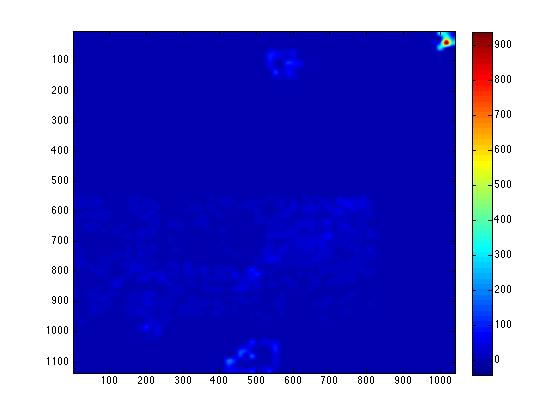
\includegraphics[width=1.1\textwidth]{src_with_airport.jpg}
      \end{subfigure}\quad
      \begin{subfigure}{0.48\textwidth}
	\caption{Distribution of Request Source without Airport}
      \centering
      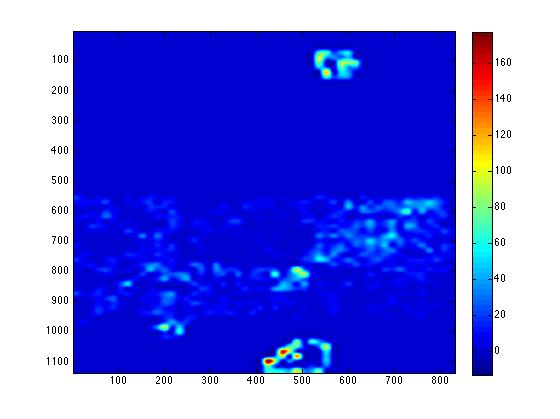
\includegraphics[width=1.1\textwidth]{src_without_airport.jpg}
      \end{subfigure}
      \begin{subfigure}{0.48\textwidth}
	\caption{Distribution of Request Destination with Airport}
      \centering
      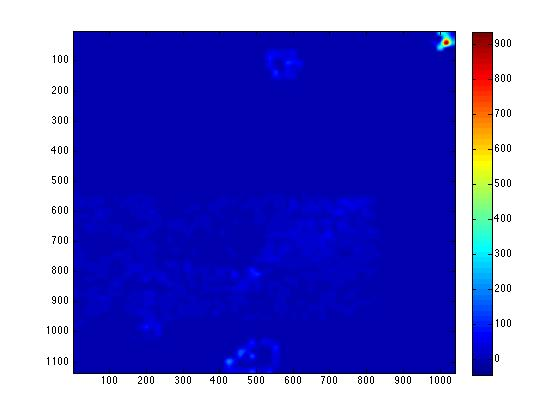
\includegraphics[width=1.1\textwidth]{dest_with_airport.jpg}
      \end{subfigure}\quad
      \begin{subfigure}{0.48\textwidth}
	\caption{Distribution of Request Destination without Airport}
      \centering
      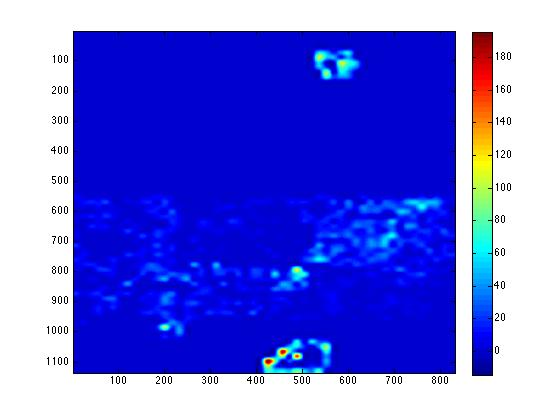
\includegraphics[width=1.1\textwidth]{dest_without_airport.jpg}
      \end{subfigure}
 \end{figure}

$$p_{unreg} = k \ln (t_{reg})$$
$$\frac{p_{unreg'}}{p_{unreg}}  = \frac{\ln_{t_{reg}}}{ \ln{t_{reg'}}}$$

\begin{center}
\begin{tabular}{ | c | c | c | c | c | c | c | c | c | }
\hline
 Number of Cabs & 14 & 15 & 16 & 17 & 18 & 19 & 20 & 21 \\\hline
Uni Ind/Conglo & 1.5720  &  1.3773  &  1.2880 &   1.2071 &   1.1932 &  1.2113  &  1.1201  &  1.0672\\\hline
Prop Ind/Conglo & 1.6876  &  1.4040  &  1.2459  &  1.1248  &  1.2558  &  1.1498  &  1.1033  &  1.1022\\\hline
Disprop Ind/Conglo & 2.1519  &  2.0706 &   2.0489  &  1.9399  &  1.8725 &   1.8174  &  1.6990 &   1.3905\\
\hline
\end{tabular}
\end{center}

\section{Strengths and Weaknesses}
\subsection{Strengths}
\begin{itemize}
\item Todo
\end{itemize}
\subsection{Weaknesses}
\begin{itemize}
\item Todo
\end{itemize}

\section{Conclusions}
Todo

\section{Future work}
\begin{itemize}
\item Todo
\end{itemize}

\pagebreak

\section{Bibliography}
\begin{thebibliography}{9}

\bibitem{OSM} OpenStreetMaps API,
\verb|http://www.openstreetmap.org/#map=14/42.4427/-76.4984|
\bibitem{Gist} Github Gist by user aflaxman,
\verb|https://gist.github.com/aflaxman/287370/|
\bibitem{Re} $\text{A stochastic optimization model for real-time ambulance redeployment}$,
\\\verb|http://www.sciencedirect.com/science/article/pii/S0305054813000385|
\bibitem{Ithaca} Ithaca Demographics,
\verb|http://www.ci.ithaca.ny.us/maps/index.cfm|
\bibitem{Cornell} Cornell Demographics,
\verb|http://www.cornell.edu/about/facts/stats.cfm|
\bibitem{IC} Ithaca College,
\verb|http://www.ithaca.edu/admission/facts/|


\end{thebibliography}

\pagebreak

\section{Code}


\definecolor{mygreen}{rgb}{0,0.6,0}
\definecolor{mygray}{rgb}{0.5,0.5,0.5}
\definecolor{mymauve}{rgb}{0.58,0,0.82}

\lstset{ %	
  backgroundcolor=\color{white},   % choose the background color; you must add \usepackage{color} or \usepackage{xcolor}
  basicstyle=\footnotesize,        % the size of the fonts that are used for the code
  breakatwhitespace=false,         % sets if automatic breaks should only happen at whitespace
  breaklines=true,                 % sets automatic line breaking
  captionpos=b,                    % sets the caption-position to bottom
  commentstyle=\color{mygreen},    % comment style
  deletekeywords={...},            % if you want to delete keywords from the given language
  escapeinside={\%*}{*)},          % if you want to add LaTeX within your code
  extendedchars=true,              % lets you use non-ASCII characters; for 8-bits encodings only, does not work with UTF-8
  frame=single,                    % adds a frame around the code
  keepspaces=true,                 % keeps spaces in text, useful for keeping indentation of code (possibly needs columns=flexible)
  keywordstyle=\color{blue},       % keyword style
  morekeywords={*,...},            % if you want to add more keywords to the set
  numbers=left,                    % where to put the line-numbers; possible values are (none, left, right)
  numbersep=5pt,                   % how far the line-numbers are from the code
  numberstyle=\tiny\color{mygray}, % the style that is used for the line-numbers
  rulecolor=\color{black},         % if not set, the frame-color may be changed on line-breaks within not-black text (e.g. comments (green here))
  showspaces=false,                % show spaces everywhere adding particular underscores; it overrides 'showstringspaces'
  showstringspaces=false,          % underline spaces within strings only
  showtabs=false,                  % show tabs within strings adding particular underscores
  stepnumber=2,                    % the step between two line-numbers. If it's 1, each line will be numbered
  stringstyle=\color{mymauve},     % string literal style
  tabsize=2,                       % sets default tabsize to 2 spaces
  title=\lstname,                  % show the filename of files included
  columns=fullflexible,basicstyle=\ttfamily,  
  language=Python    
}
\begin{lstlisting}[frame=none]
\end{lstlisting}

\end{document}